\PID\mnImportant
Поједноставити следеће изразе 
(а) $\updelta(at)$, и
(б) $\int_{-\infty}^{\infty} x(t)\updelta(t-\uptau)\de t$, 
где су $a, \uptau \in \mathbb R$ познати реални параметри, а $x(t)$ је непрекидан сигнал.

\RESENJE
Строга анализа Дираковог импулса\footnote{Поред овог назива који ће бити коришћен у овом тексту, присутни су и 
делта импулс, Дираков делта импулс, Диракова делта \textit{функција}. Пошто овај математички објект строго није функција, 
тај назив ћемо избегавати.} захтева залажење у математичку теорију дистрибуција. Ипак, за инжењерске потребе, овај импулс
има изузетан значај и биће присутан кроз цео наставак ове збирке. Ми ћемо га третирати на инжењерски начин, полазећи од његова 
два основна својства, и то 
\begin{eqnarray}
    && \int_{-\infty}^{\infty} \updelta(t)\,\de t = 1\text{, и} \label{eq:dirak_def:1} \\
    && \updelta(t \neq 0) = 0 \label{eq:dirak_def:2}
\end{eqnarray}
Ова два услова су, гледано са становишта класичне математичке анализе, противречна. Не постоји таква функција да је 
равна нули у свим тачкама осим једне, а да је њен интеграл различит од нуле. Ипак, уколико кажемо да је понашање 
Делта импулса у околини нуле „необично“ (недефинисано), онда можемо доћи до веома корисних закључака. На пример, 
посматрајмо правоугаони импулс који се произвољно сужава, при чему се његова амплитуда повећава тако да његова 
површина остаје јединична. Такав сигнал назовимо језгром Делта импулса $\updelta_a(t) = \dfrac{1}{a}
\rect\left(\dfrac{t}{a}\right)$, где је $a$ реални параметар који описује ширину импулса. Уколико 
узмемо да произвољно смањујемо ширину $a$ можемо да закључимо да је увек $\int_{-\infty}^{\infty} \updelta_a(t)\de t = 1$
за свако $a$, а да постепено само језгро постаје све „концентрисаније“ око нуле, односно да тим процесом све вредности 
осим нуле теже нули. Такође, то не зависи од иницијално одабира језгра, слично би се десило и са јединичним троугаоним 
и са јединичним $\sinc$ сигналом. Резултат тог процеса јесте Дираков импулс, као што је илустровано на слици: 
\begin{figure}[ht!]
    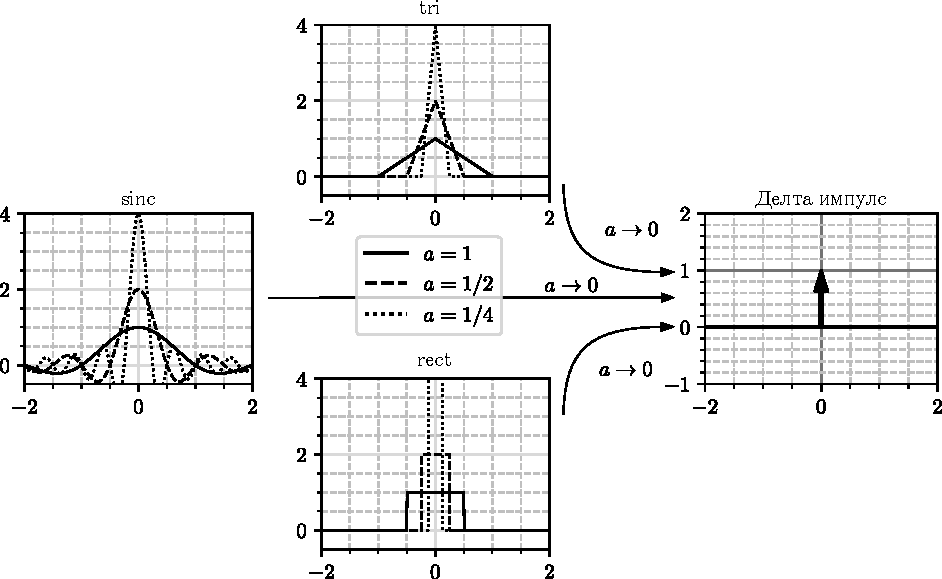
\includegraphics[width=\textwidth]{fig/dirac_kernel.pdf}
    \caption{Илустрација процеса настајања Дираковог импулса. Језгро одабрано полазећи од три различита јединична сигнала, 
    процесом $a\to0$ постаје Дираков импулс.}
\end{figure}

\noindent
Може се писати и $\updelta(t) = \lim_{a\to 0} \updelta_a(t)$, али треба бити пажљив када је употреба овог израза у питању,
јер гранична вредност није дефинисана у нули. Када год се анализира утицај Дираковог импулса, треба размишљати о утицају
било ког језгра Делта импулса, па уочити шта се дешава када се спроведе описани гранични процес. 

(а) Анализу $\updelta(at)$ ћемо спровести на основу дефиниционих релација \eqref{eq:dirak_def:1} и \eqref{eq:dirak_def:2},
пре свега, размотримо интеграл $\int_{-\infty}^{\infty} \updelta(at) \de t$, који се може решити сменом 
$u = at \Rightarrow \de u = a \de t$. Том приликом, треба повести рачуна да су у случају када је $a<0$ границе интеграције окренуте, па је онда 
\begin{equation}
    \int_{-\infty}^{\infty} \updelta(at) \de t = 
    \int_{\-\infty}^{\infty} \updelta(u) \dfrac{\de u}{a} 
    = 
    \begin{cases}
    \dfrac{1}{a} \,\, \cancelto{1}{\int_{-\infty}^{\infty} \updelta(u) \de u} &, a > 0, \\
    \dfrac{1}{a} \,\, \cancelto{-1}{\int_{\infty}^{-\infty} \updelta(u) \de u} &, a < 0
    \end{cases}
    = \dfrac{1}{|a|}.
\end{equation}
Такође, приметимо да је $\updelta(at \neq 0) = 0$ еквивалентно са $\updelta(t \neq 0) = 0$ па је тиме задовољен и 
услов \eqref{eq:dirak_def:2}. Коначно, закључујемо да сигнал $\updelta(at)$ има површину $1/|a|$ док је раван нули свуда
осим за $t=0$, то значи да се може писати: 
\begin{equation}
    \updelta(at) = \dfrac{1}{|a|} \updelta(t), 
\end{equation}
што се назива својством скалирања Делта импулса. 

(б) У датом интегралу  $\int_{-\infty}^{\infty} x(t)\updelta(t-\uptau)\de t$ јавља се Делта импулс 
померен на тренутак $t = \uptau$. Овај проблем можемо третирати раздвајањем овог интеграла на три дела, издвајајући 
инфинитезималну околину $[\uptau^-, \uptau^+]$ на тај начин, 
\begin{equation}
    \int_{-\infty}^{\infty} x(t)\updelta(t-\uptau)\de t = 
    \cancelto{0}{\int_{-\infty}^{\uptau^-} x(t)\updelta(t-\uptau)\de t} + 
    \int_{\uptau^-}^{\uptau^+} x(t)\updelta(t-\uptau)\de t +
    \cancelto{0}{\int_{\uptau^+}^{\infty} x(t)\updelta(t-\uptau)\de t}
\end{equation}
Први и трећи интеграл равни су нули јер је домен интеграције ван непосредне околине вредности $t = \uptau$ па су 
Диракови импулси у тим интегралима увек равни нули. Средњи интеграл, у околини те вредности, решићемо знајући да је 
$x(t)$ непрекидан сигнал. Наиме, пошто се разматра произвољно уска околина око параметра $\uptau$ то се може писати 
да је $x(\uptau^- < t < \uptau^+) \to x(\uptau)$, односно сигнал $x(t)$ је на том интервалу практично константа, па је 
\begin{equation}
    \int_{\uptau^-}^{\uptau^+} x(t)\updelta(t-\uptau)\de t 
    =
    \int_{\uptau^-}^{\uptau^+} \underbrace{x(\uptau)}_{\rm const}\updelta(t-\uptau)\de t 
    =
    x(\uptau) \cancelto{1}{\int_{\uptau^-}^{\uptau^+} \updelta(t-\uptau)\de t}
    =
    x(\uptau).
\end{equation}
Добијени резултат представља веома важно тзв. \emph{својство одабирања} или \emph{својство селекције} 
Дираковог импулса: 
\begin{eqnarray}
    \int_{-\infty}^{\infty} x(t)\updelta(t-\uptau)\de t = x(\uptau).
\end{eqnarray}
